% Options for packages loaded elsewhere
\PassOptionsToPackage{unicode}{hyperref}
\PassOptionsToPackage{hyphens}{url}
%
\documentclass[
]{article}
\usepackage{amsmath,amssymb}
\usepackage{iftex}
\ifPDFTeX
  \usepackage[T1]{fontenc}
  \usepackage[utf8]{inputenc}
  \usepackage{textcomp} % provide euro and other symbols
\else % if luatex or xetex
  \usepackage{unicode-math} % this also loads fontspec
  \defaultfontfeatures{Scale=MatchLowercase}
  \defaultfontfeatures[\rmfamily]{Ligatures=TeX,Scale=1}
\fi
\usepackage{lmodern}
\ifPDFTeX\else
  % xetex/luatex font selection
\fi
% Use upquote if available, for straight quotes in verbatim environments
\IfFileExists{upquote.sty}{\usepackage{upquote}}{}
\IfFileExists{microtype.sty}{% use microtype if available
  \usepackage[]{microtype}
  \UseMicrotypeSet[protrusion]{basicmath} % disable protrusion for tt fonts
}{}
\makeatletter
\@ifundefined{KOMAClassName}{% if non-KOMA class
  \IfFileExists{parskip.sty}{%
    \usepackage{parskip}
  }{% else
    \setlength{\parindent}{0pt}
    \setlength{\parskip}{6pt plus 2pt minus 1pt}}
}{% if KOMA class
  \KOMAoptions{parskip=half}}
\makeatother
\usepackage{xcolor}
\usepackage[margin=1in]{geometry}
\usepackage{graphicx}
\makeatletter
\newsavebox\pandoc@box
\newcommand*\pandocbounded[1]{% scales image to fit in text height/width
  \sbox\pandoc@box{#1}%
  \Gscale@div\@tempa{\textheight}{\dimexpr\ht\pandoc@box+\dp\pandoc@box\relax}%
  \Gscale@div\@tempb{\linewidth}{\wd\pandoc@box}%
  \ifdim\@tempb\p@<\@tempa\p@\let\@tempa\@tempb\fi% select the smaller of both
  \ifdim\@tempa\p@<\p@\scalebox{\@tempa}{\usebox\pandoc@box}%
  \else\usebox{\pandoc@box}%
  \fi%
}
% Set default figure placement to htbp
\def\fps@figure{htbp}
\makeatother
\setlength{\emergencystretch}{3em} % prevent overfull lines
\providecommand{\tightlist}{%
  \setlength{\itemsep}{0pt}\setlength{\parskip}{0pt}}
\setcounter{secnumdepth}{-\maxdimen} % remove section numbering
\PassOptionsToPackage{top=0.2in, bottom=0.2in, left=0.5in, right=0.5in}{geometry}
\pagestyle{empty}
\usepackage{graphicx}
\usepackage{float}
\raggedbottom
\usepackage{bookmark}
\IfFileExists{xurl.sty}{\usepackage{xurl}}{} % add URL line breaks if available
\urlstyle{same}
\hypersetup{
  hidelinks,
  pdfcreator={LaTeX via pandoc}}

\author{}
\date{\vspace{-2.5em}}

\begin{document}

\vspace*{-8em}
\begin{center}
\vspace*{-1em}
\LARGE \textbf{KCL Umpire Report}
\vspace*{-1em}
\end{center}

\begin{center}
\begin{minipage}{0.28\textwidth}
\centering
\Large \textbf{REX vs NOR}
\end{minipage}
\hfill
\begin{minipage}{0.28\textwidth}
\centering

\includegraphics[width=\textwidth]{ump-mask.png}
\end{minipage}
\hfill
\begin{minipage}{0.28\textwidth}
\centering
\Large 07/26
\end{minipage}
\vspace*{-1em}
\end{center}

\begin{center}
\centering
\vspace{1em}
\Large \textbf{Overall Accuracy}
\end{center}

\begin{center}
\begin{minipage}[t][3.5in][t]{\textwidth}
\begin{minipage}[t]{0.25\textwidth}
\centering
\vspace*{-5em}
\textbf{Called 158 out of}
\textbf{195 taken pitches correctly}
\end{minipage}
\hfill
\begin{minipage}[t]{0.28\textwidth}
\centering
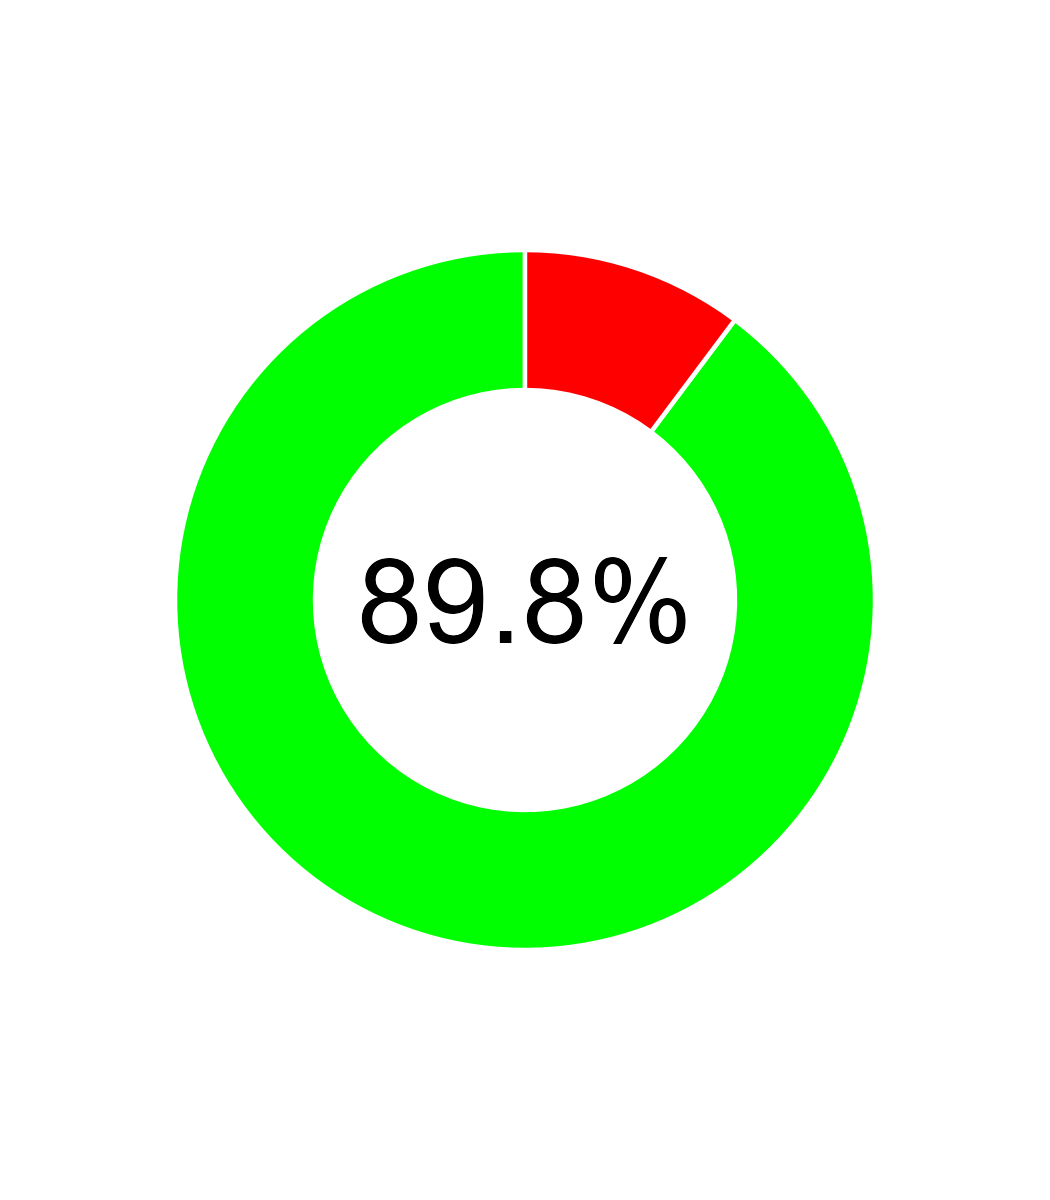
\includegraphics[width=0.8\textwidth]{plots/overall_accuracy.png}
\end{minipage}
\hfill
\begin{minipage}[t]{0.25\textwidth}
\centering
\vspace*{-4em}
\textbf{KCL Accuracy Percentile: 44}
\end{minipage}
\end{minipage}
\end{center}

\vspace*{-15em}

\begin{center}
\Large \textbf{All Missed Calls}
\end{center}

\begin{center}
\begin{minipage}[t]{0.3\textwidth}
\centering
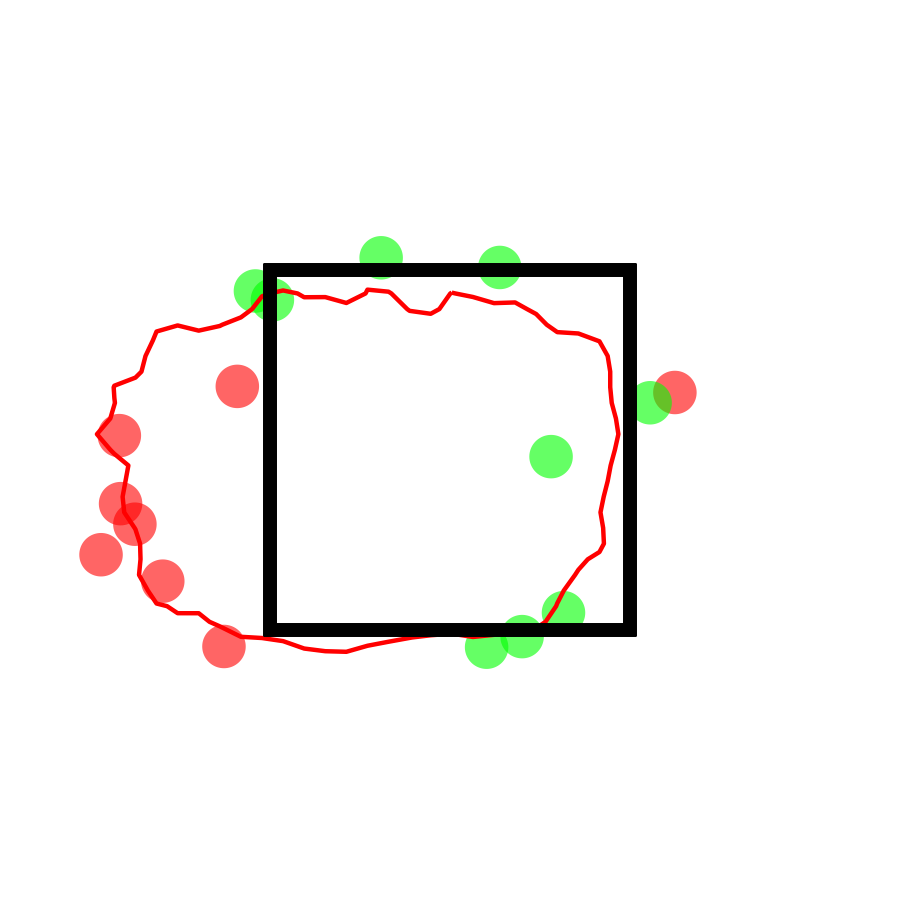
\includegraphics{plots/missed_calls.png}
\end{minipage}
\hfill
\begin{minipage}[t]{0.2\textwidth}
\centering

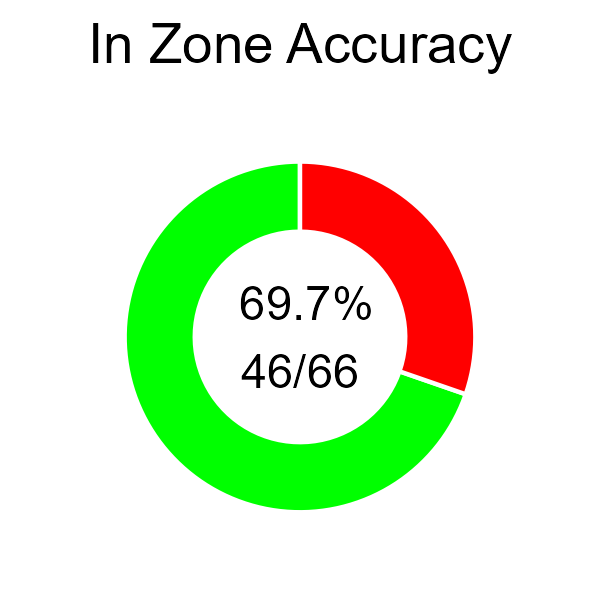
\includegraphics{plots/iz_accuracy.png}
\end{minipage}
\hfill
\begin{minipage}[t]{0.2\textwidth}
\centering

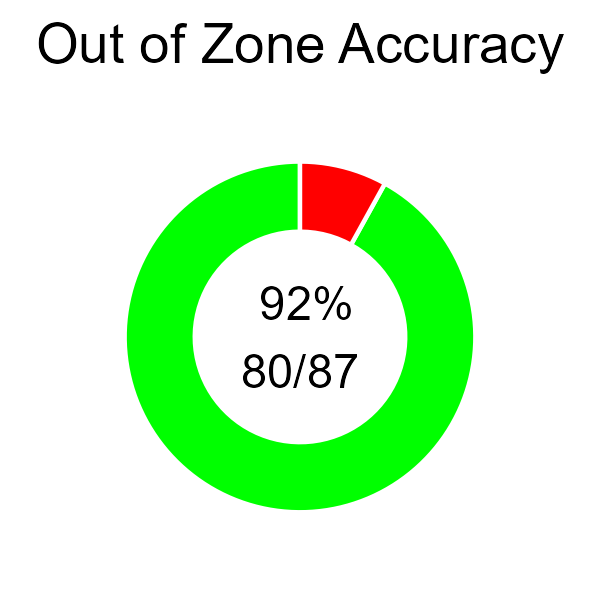
\includegraphics{plots/oz_accuracy.png}
\end{minipage}
\end{center}

\end{document}
